\documentclass{article}

% Chinese Support using xeCJK
% \usepackage{xeCJK}
%\setCJKmainfont{SimSun}

% Chinese Support using CTeX
% \usepackage{ctex}

% Math Support
\usepackage{amsmath}
\usepackage{amsfonts}
\usepackage{amssymb}
\usepackage{wasysym}
\newcommand{\angstrom}{\text{\normalfont\AA}}

% Graphics Support
\usepackage{graphicx}
\usepackage{float}

% Reduced page margin
\usepackage{geometry}
\geometry{a4paper,scale=0.8}

\usepackage{caption}
\usepackage{subcaption}

% d and e should be math operators
\newcommand*{\dif}{\mathop{}\!\mathrm{d}}
\newcommand*{\md}{\mathop{}\!\mathrm{d}}
\newcommand*{\me}{\mathrm{e}}

% No indent for each paragraph
\usepackage{parskip}
\setlength{\parindent}{0cm}

% Bold style for Greek letters
\usepackage{bm}
\let\Oldmathbf\mathbf
\renewcommand{\mathbf}[1]{\boldsymbol{\Oldmathbf{#1}}}

% More space for dfrac in cell
\usepackage{cellspace}
\setlength{\cellspacetoplimit}{5pt}
\setlength{\cellspacebottomlimit}{5pt}

% SI units
\newcommand{\si}[1]{\  \mathrm{#1}}

% Multi-line author information
\usepackage{authblk}
\author{Xiping Hu}
\affil{https://hxp.plus/}

\title{Homework for Chapter 10}

\begin{document}

\maketitle

\begin{figure}[H]
  \centering
  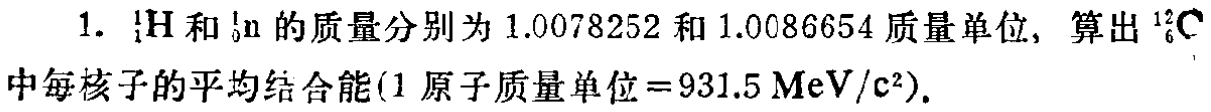
\includegraphics[width=\linewidth]{figures/Problem1}
  \label{fig:}
\end{figure}

\begin{equation*}
  \begin{aligned}
    \Delta \bar{E} = \left[ 6 m_H + 6 m_n - 12 m_A \right] c^2 / 12 = 7.6805 \si{MeV}
   \end{aligned}
\end{equation*}

\begin{figure}[H]
  \centering
  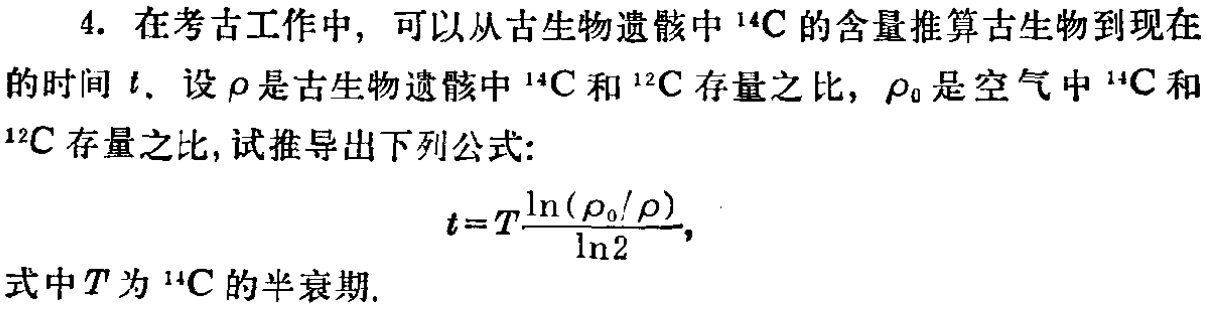
\includegraphics[width=\linewidth]{figures/Problem4}
  \label{fig:}
\end{figure}

\begin{equation*}
  \begin{aligned}
    \dfrac{\rho}{\rho_0} = \dfrac{1}{2}^{t/T} \quad\quad \Rightarrow \quad\quad
    \dfrac{\rho_0}{\rho} = 2^{t/T} \quad\quad \Rightarrow \quad\quad
    \ln \left( \rho_0 / \rho \right) = \dfrac{t}{T} \ln 2 \quad\quad \Rightarrow \quad\quad
    t = T \dfrac{\ln \left( \rho_0 / \rho \right)}{\ln 2} 
  \end{aligned}
\end{equation*}

\begin{figure}[H]
  \centering
  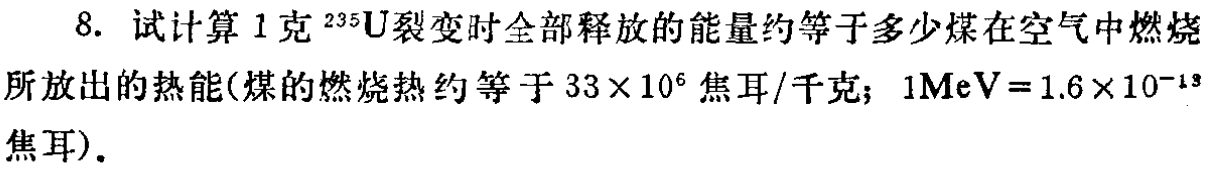
\includegraphics[width=\linewidth]{figures/Problem8}
  \label{fig:}
\end{figure}

\begin{equation*}
  \begin{aligned}
    \Delta E = 236 \times \left( 8.5 - 7.6 \right) = 212.4 \si{MeV} = 3.40302 \times 10^{-11} \si{J}
  \end{aligned}
\end{equation*}

\begin{equation*}
  \begin{aligned}
    E = \dfrac{m N_A}{M_U} \cdot \Delta E = 8.71753 \cdot 10^{10} \si{J}
  \end{aligned}
\end{equation*}

\begin{equation*}
  \begin{aligned}
    m_{coal} = \dfrac{E}{33 \times 10^6} =  2641.68 \si{kg}
  \end{aligned}
\end{equation*}

\end{document}